\documentclass[preview]{standalone}

\usepackage{amsmath}
\usepackage{amssymb}
\usepackage{stellar}
\usepackage{bettelini}
\usepackage{wrapfig}

\hypersetup{
    colorlinks=true,
    linkcolor=black,
    urlcolor=blue,
    pdftitle={Biologia},
    pdfpagemode=FullScreen,
}

\begin{document}

\title{Biologia}
\id{biologia-apparato-circolatorio}
\genpage

\section{Apparato circolatorio}

\begin{snippetdefinition}{sistema-circolatorio-definition}{Sistema circolatorio}
    Il \textit{sistema circolatorio} umano è un sistema chiuso
    che trasporta il sangue, contenente varie sostanze, in giro nell'organismo pluricellulare.
\end{snippetdefinition}

\begin{snippet}{sistema-circolatorio-expl1}
    Nel caso di organismi primitivi, per cui non abbastanza complessi da necessitare un sistema circolatorio,
    non è necessario o possibile averne uno.
    L'organismo semplice è a contatto con l'ambiente e scambi energia sul momento.

    L'apparato circolatorio svolge i seguenti ruoli:
    \begin{itemize}
        \item \textbf{Trasporto:} 
        \begin{itemize}
            \item di \textit{gas} (O\({}_2\), CO\({}_2\)) trasporto passivo, diffusione semplice, polmoni \(\iff\) sangue;
            \item di \textit{metaboliti} (molecole del metabolismo), fra \(\iff\) (muscoli, reni, intestino dove vengono assorbiti, fegato dove vengono scartati);
            \item di \textit{ormoni}, cellule o ghiandole endocrine, servono come segnale e raggiungono il proprio bersaglio. % es cellula G
        \end{itemize}
        \item \textbf{Omeostasi:} mantenere alcuni parametri costanti (omeostasi), quali
            \begin{itemize}
                \item \textit{temperatura} (termoregolazione);
                \item \textit{equilibrio idrico} (idroregolazione), modificato la concentrazione dei soluti del sangue influenzando l'osmosi;
                \item il \textit{pH}, grazie all'aggiunta di sostanze acide o basiche.
            \end{itemize}
        \item \textbf{Difesa:} contiene alcune sostanze per la difesa del corpo umano, quali:
            \begin{itemize}
                \item \textit{globuli bianchi}, per distruggere organismi patogeni;
                \item \textit{anticorpi}, proteine per immobilizzare i patogeni;
                \item \textit{agenti coagulanti} (es. fibrina e piastrina), per riparare le ferite.
            \end{itemize}
    \end{itemize}

    Il sistema cardiocircolatorio umano è composto nella seguente maniera:
    \begin{itemize}
        \item \textbf{sangue:} fluido circolante (plasma + elementi cellulari);
        \item \textbf{sistema di vasi:} arterie, arteriole, vene, venule e capillari;
            Le vene riportano il sangue al cuore mentre le arterie introducono quello ossigenato.
            I capillari sono dei tubi molto piccoli nei tessuti dove avviene lo scambio fra sangue e tessuto;
        \item \textbf{cuore:} pompa, motore che permette circolazione del sangue.
            \begin{itemize}
                \item diviso in due parti separati, ciascuna con 2 cavità, un'entrata e un'uscita;
                \item circolazione sistemica e polmonare separate;
                \item cuore più performance (grazie alla separazione in 4);
                \item soddisfa elevate necessità metaboliche.
            \end{itemize}
    \end{itemize}
\end{snippet}

\plain{Il sangue è composta da una parte cellulare (45\% volume) ed una plasmatica.}

\includesnpt[width=80\%|src=/snippet/static/blood-composition.png]{centered-img}

\section{Evoluzioni nei vertebrati}

\includesnpt[width=75\%|src=/snippet/static/circulation-evolution.png]{centered-img}

\section{Anatomia del cuore}

\includesnpt[width=70\%|src=/snippet/static/heart.png]{centered-img}

\begin{snippet}{fe11ed70-afd6-469a-8070-2a9107327646}
    Il ventricolo sinistro è più grosso perché spinge il sangue ossigenato in tutto il corpo,
    mentre il ventricolo destro spinge solamente verso il polmone, il quale, è relativamente vicino.
    
    Le 4 camere si chiamano atri e ventricoli.
    Dall'atrio al ventricolo abbiamo una valvola che si chiude quando il sangue fluisce
    per evitare un reflusso (valvole atrioventricolari destra e sinistra).
    
    Dal ventricolo sinistro arriviamo all'aorta, ossia l'arteria principale.
    Una volta giunto ai tessuti, il sangue ritorna mediante una vena al cuore.
    Le vene che entrano a destra sono 2 (una dalla parte inferiore del corpo, e una dalla parte superiore).
    Queste due vene si chiamano \textit{vena cava inferiore} e \textit{vena cava superiore}.
    La vena che porta il sangue ossigenato al cuore si chiama vena polmonare, ed entra nell'atrio sinistro.
    
    %%%%%%%%%%%%%%%%%%%%%%%%%%% schemino circolazione nei mammiferi
    
    I nutrienti vengono caricati nel sangue, per cui tutta la circolazione polmonare e sistemica
    è anche ricca di nutrienti. Nella vena cava inferiore vi è molto nutrimento
    (come tutte le vene che vi ci uniscono), mentre nella vena cava superiore ve ne sono pochi.

    % schema valcole valcole semilunari e atrioventricolari
\end{snippet}

\section{Struttura dei vasi sanguigni}

\begin{snippet}{4f960dbc-10eb-4300-b62e-511275979e30}
    I capillari hanno pareti molto sottili, costituite da un singolo strato di cellule epiletali.
    Arterie, arteriole, vene e venule hanno pareti più spesse, rivestite da un epitelio e rinforzate da uno strato di tessuto muscolare liscio e da uno di tessuto connettivo.
\end{snippet}

% schema

\section{Ciclo cardiaco}

\begin{snippet}{ciclo-cardiaco-expl1}
    Il ciclo cardiaco, a riposo, dura 0.8 secondi (75 bpm).
    Nella diastole, per la durata 0.4 secondi, tutto il cuore si rilassa.
    Durante questo periodo il sangue fluisce.
    Successivamente avviene la contrazione degli atri (sistole atriale di 0.1 secondi).
    Infine, la fase di sistole ventricolare spinge il sangue nelle arterie (0.3 secondi).
    Questo ciclo avviene in ambo le parti del cuore con uno sfasamento di mezzo periodo.
\end{snippet}

\section{Regolazione del ritmo cardiaco}

\begin{snippet}{ciclo-cardiaco-expl2}
    Il segnale elettrico è quando il potenziale di membrana viene invertito.
    Le cellule adiacenti comunicano quindi invertendo questo segnale (dentro positivo e fuori negativo, e viceversa),
    stimolandosi a vicenda e depolarizzandosi.
    I segnali elettrici che insorgono e si propagano nel cuore generano dei
    cambiamenti elettrici sulla pelle che possono essere rilevati tramite degli
    elettrodi e registrati come elettrocardiogramma (ECG).
    
    L'impulso elettrico nasce nel atrio destro nel nodo chiamato seno-atriale (pacemaker).
    Il segnale si propaga lungo le fibre muscolari specializzate.
    
    % 1) depolarizzazione atrio, 2) depolarizzazione ventricolo, 3) ripolarizzazione ventricoli
\end{snippet}

\includesnpt[width=85\%|src=/snippet/static/pacemaker.png]{centered-img}

\section{Circolazione coronarica}

\includesnpt[width=70\%|src=/snippet/static/circolazione-coronarica.png]{centered-img}

\plain{Le vene coronariche vanno ad alimentare il muscolo del cuore.}

\section{Aterosclerosi}

\begin{snippetdefinition}{Aterosclerosi-definition}{Aterosclerosi}
    L'\textit{ateroscelrosi} è una malattia che implica la formazione di placche (ateromi) all'interno delle pareti delle arterie.
\end{snippetdefinition}

\plain{Il lume si restringe e lo scorrimento del sangue diventa difficoltoso.
La causa principale è l'eccesso di colesterolo.}

\section{Pressione sanguigna}

\begin{snippetdefinition}{pressione-sanguigna-definition}{Pressione sanguigna}
    La \textit{pressione sanguigna} è la pressione esercitata dal cuore.
\end{snippetdefinition}

\begin{snippet}{352be194-4d29-4afa-862d-08159fee41a3}
    \setlength{\intextsep}{0pt}%
    \begin{wrapfigure}{l}{8cm}
        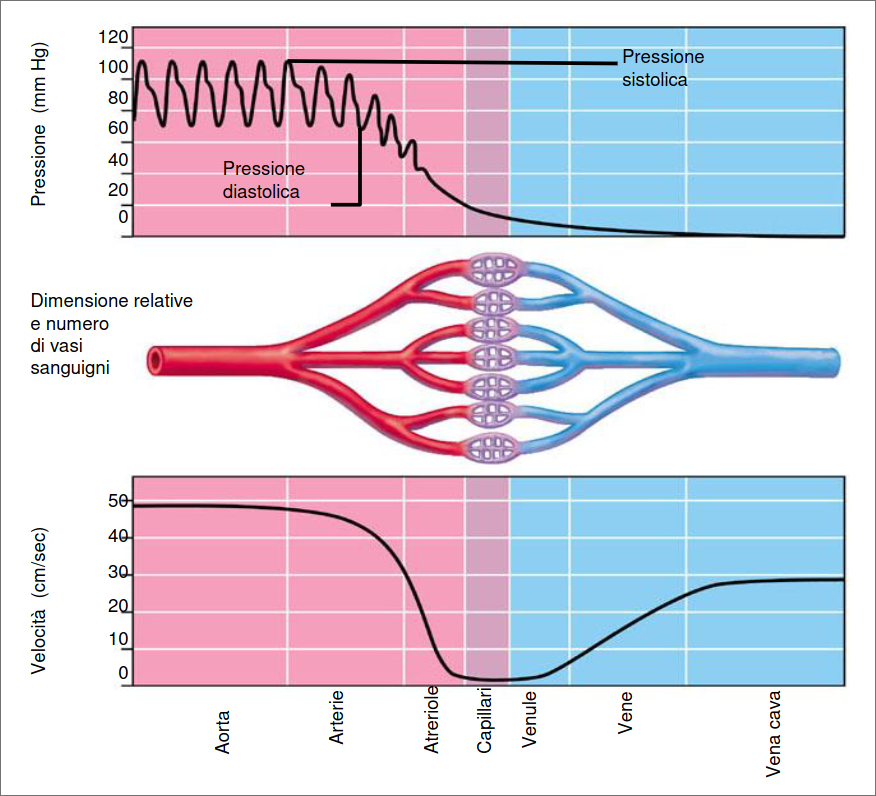
\includegraphics[width=7.5cm]{./resources/pressione.png}
        \vspace{-1cm}
    \end{wrapfigure}
    
    La pressione sanguigna diminuisce più ci si allontana dal cuore, e diventa minima ai capillari.
    Vi sono in realtà 2 pressioni:
    quella sistolica (valore massimo, quando il ventricolo si contrae) e quella diastolica
    (valore minimo, quando il vaso sanguigno si dilata e successivamente si richiude, dando una spinta).
    
    Il valore normale della pressione sanguigna di un adulto è 120/70 (mmHg / mmHg).
    Essa di misura con uno sfigmomanometro.
    
    I muscoli scheletrici permettono al sangue di ritornare al cuore dopo i capillari.
    Essi schiacciano il vaso spinegendo il sangue verso il cuore.
    % si ferma per favorire lo scambio ai capillari
    \wrapfill
\end{snippet}

\end{document}